% 2007 上海文 Q21 图: “果圆”
% 右半椭圆 x^2/a^2+y^2/b^2=1 (x>=0) 与左半椭圆 y^2/b^2+x^2/c^2=1 (x<=0), a^2=b^2+c^2, a>b>c>0。
% 取源图比例(等边三角形情形): a=sqrt7/2, b=1, c=sqrt3/2, d=sqrt(b^2-c^2)=1/2。
% 焦点 F0(c,0), F1(0,-d), F2(0,d); 交点 A1(-c,0), A2(a,0), B1(0,-b), B2(0,b); M 为 A1A2 中点。
\usetikzlibrary{arrows.meta,calc}
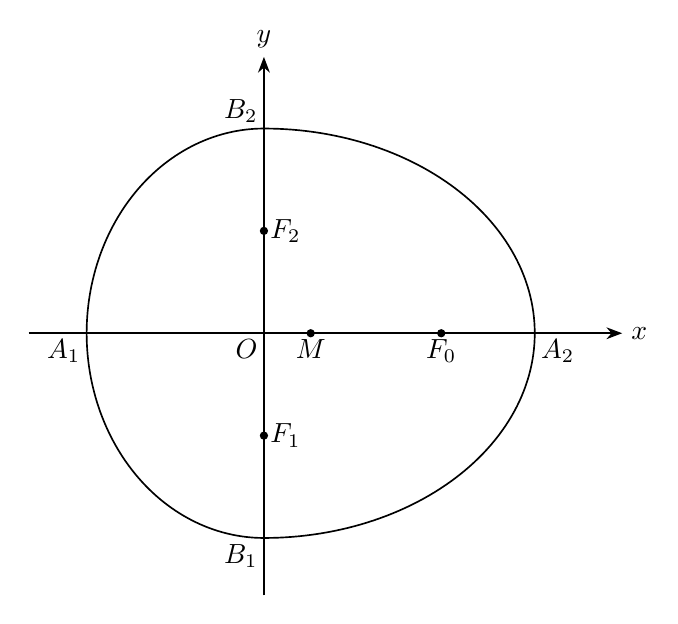
\begin{tikzpicture}[x=2.6cm,y=2.6cm,line width=.6pt,font=\normalsize,>=Stealth,
  lbl/.style={inner sep=1pt}]
\def\a{1.3228756555}
\def\b{1}
\def\c{0.8660254038}
\coordinate (O) at (0,0);
\coordinate (A1) at (-\c,0);
\coordinate (A2) at (\a,0);
\coordinate (B1) at (0,-\b);
\coordinate (B2) at (0,\b);
\coordinate (F0) at (\c,0);
\coordinate (F1) at (0,-0.5);
\coordinate (F2) at (0,0.5);
\coordinate (M) at (0.2284251259,0);
% 右半椭圆 (t in [-90,90]) 与左半椭圆 (t in [90,270])
\draw[domain=-90:90,samples=121,variable=\t] plot ({\a*cos(\t)},{\b*sin(\t)});
\draw[domain=90:270,samples=121,variable=\t] plot ({\c*cos(\t)},{\b*sin(\t)});
\draw[->] (-1.15,0)--(1.75,0) node[lbl,right,xshift=2pt] {$x$};
\draw[->] (0,-1.28)--(0,1.35) node[lbl,above,yshift=2pt] {$y$};
\fill (F0) circle (1.5pt);
\fill (F1) circle (1.5pt);
\fill (F2) circle (1.5pt);
\fill (M) circle (1.5pt);
\node[anchor=north east,inner sep=0pt,xshift=-2pt,yshift=-2pt] at (O) {$O$};
\node[anchor=north east,inner sep=0pt,xshift=-2pt,yshift=-2pt] at (A1) {$A_1$};
\node[anchor=north west,inner sep=0pt,xshift=2pt,yshift=-2pt] at (A2) {$A_2$};
\node[anchor=north east,inner sep=0pt,xshift=-2pt,yshift=-2pt] at (B1) {$B_1$};
\node[anchor=south east,inner sep=0pt,xshift=-2pt,yshift=2pt] at (B2) {$B_2$};
\node[anchor=west,inner sep=0pt,xshift=2pt] at (F2) {$F_2$};
\node[anchor=west,inner sep=0pt,xshift=2pt] at (F1) {$F_1$};
\node[anchor=north,inner sep=0pt,yshift=-2pt] at (F0) {$F_0$};
\node[anchor=north,inner sep=0pt,yshift=-2pt] at (M) {$M$};
\end{tikzpicture}
